\noindent Một bình kín được chia thành 3 phần,$A$, $B$ và $C$ bởi hai vách ngăn $D_1$ và $D_2$ như được biểu diễn trên hình 2.1. Mỗi phần được lấp đầy bởi một lượng khí lí tưởng đơn nguyên tử có áp suất $P$, thể tích $V$ và nhiệt độ tuyệt đối $T$ như được chỉ ra trên hình vẽ. Vách ngăn $D_1$ có khối lượng $m$ và có thể di chuyển tự do không ma sát, trong khi đó, vách ngăn $D_2$ được gắn cố định và có một van nhỏ được gắn trên nó. Mở van, khí trong phần $B$ và $C$ hoà làm một và hệ tiến tới trạng thái cân bằng trong khi vẫn duy trì nhiệt độ $T_0$.
\begin{figure}[h]
  \centering
  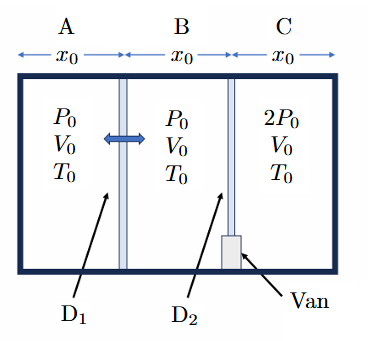
\includegraphics[width=0.5\textwidth]{Figures/Problems/Fig 2.1.png}
  \begin{center}
    \figurename{ 2.1}
  \end{center}
\end{figure}

\begin{enumerate}
  \item Xác định áp suất và thể tích của khí trong các phần $A, B$ và $C$ khi hệ đạt trạng thái cân bằng.
  \item Tính nhiệt lượng mà khí trong phần $B$ và $C$ đã nhận trong toàn bộ quá trình.
  \item Tính độ biến thiên entropy $\Delta S$ của hệ.
\end{enumerate}